%!TEX program = xelatex
\documentclass[12pt,a4paper]{exam-zh}

\usepackage{amsmath,array,graphicx,booktabs,multirow}
\usepackage{enumitem}
\usepackage{fancyhdr}
\usepackage{tikz}
\usepackage{tabularx}
\usepackage{setspace}
\usepackage{multicol}
\setCJKmainfont{Noto Serif CJK SC}
\geometry{margin=2.2cm,top=2.0cm,bottom=2.2cm}
\pagestyle{fancy}
\fancyhf{}
\cfoot{-\thepage{}-}
\renewcommand{\headrulewidth}{0pt}
\renewcommand{\footrulewidth}{0pt}
\setlength{\parindent}{0pt}
\setlength{\parskip}{0.2em}
\setlength{\headheight}{14pt}
\linespread{1.12}
\usepackage{setspace}
\usepackage{eso-pic}
\usetikzlibrary{calc}

%region exam setup

\examsetup{
    page = {
    size = a4paper,           % 设定纸张大小 [4]
    foot-content = { - ; - }  % 页脚显示为 -1-, -2- 格式 [3]
  },
    choices = {
    label-pos = top-left,
    column-sep = 1em,
    label-pos = auto,
    label-sep = 0.5em,
    max-columns = 4
    },
  question = {
    top-sep    = 1em, % 调整题目上方的垂直距离（默认值为 .5em plus .5em minus .2em）
    bottom-sep = 1em  % 调整题目下方的垂直距离（默认值为 .5em plus .5em minus .2em）
  },
    paren = {
    show-paren = false  % 设置为 false 则不显示括号 [3, 4]
  },
    choices = {
    label = \textbf{\Alph*}
  }, 
    solution = {
    show-solution = show-move, % 答案自动移动到卷末
    label-content = {参考答案},  % 答案区的标题文字
    show-qed = true            % 在解答末尾显示结束符号 ◻ 
  }
}

%endregion

% region 卷末参考答案改为左右双栏，题目正文不受影响
\RemoveFromHook{enddocument}[exam-zh-question]
\ExplSyntaxOn
\AddToHook{enddocument}[two-column-solutions]
  {
    \bool_if:NT \g__examzh_solution_show_move_bool
      {
        \newpage
        \begin{center}
          \zihao{-2} \heiti \makebox[5em][s]{参考答案}
        \end{center}
        \vspace*{2ex}

        \begin{center}
          \textbf{答案总表}\par
          \vspace{0.6em}
          \begin{tikzpicture}
            \pgfmathtruncatemacro{\answercols}
              {ifthenelse(\value{answerkeyquestion}<=16,8,10)}
            \pgfmathsetlengthmacro{\answerboxwidth}
              {(\linewidth-0.4pt)/\answercols}
            \pgfmathsetlengthmacro{\answerboxheight}{1.05cm}
            \pgfmathsetlengthmacro{\answeroffset}{0.12cm}
            \answerkeyitems
          \end{tikzpicture}
        \end{center}
        \vspace*{2ex}

        \setlength{\columnsep}{1cm}
        \begin{multicols}{2}
          \raggedcolumns
          \small \kaishu
          \int_compare:nNnT { \g__examzh_question_index_int } > { 0 }
            {
              \int_step_inline:nn { \g__examzh_question_index_int }
                {
                  \file_if_exist:nT { examzh #1 .solution }
                    { \file_input:n { examzh #1 .solution } }
                }
            }
        \end{multicols}
      }
  }
\ExplSyntaxOff

%endregion


%region 卷面变量设置
    % ==========================
% ==========================
% 卷面变量设置（只需改这里）
% ==========================
\newcommand{\papercode}{SC 05/SC 06}
\newcommand{\examtitle}{2026年金宝培元独立中学八月考}
\newcommand{\examlevel}{高中组}
\newcommand{\examsubject}{高级数学(I)/高级数学}
\newcommand{\sidebartext}{高级数学(I)/一}
\newcommand{\papername}{试卷一}
\newcommand{\papertype}{选择题}
\newcommand{\examdate}{2026年8月7日}
\newcommand{\examtime}{11.00 a.m. 至11.45 a.m.}
\newcommand{\examduration}{45分钟}
\newcommand{\questionpages}{4面}
\newcommand{\paperonepercentage}{40\%}
\newcommand{\papertwopercentage}{60\%}
\newcommand{\setterteacher}{蔡杰庆师}
\newcommand{\reviewteacher}{杨丽芳师}
\newcommand{\auditteacher}{雷泳健师}
\newcommand{\optrow}[4]{%
    \begin{tabular*}{\linewidth}{@{\extracolsep{\fill}}llll}
    A~#1 & B~#2 & C~#3 & D~#4
    \end{tabular*}%
}
\newcommand{\qitem}[5]{\item #1\par\optrow{#2}{#3}{#4}{#5}}

\makeatletter
\newcounter{answerkeyquestion}
\let\originalparen\paren
\newcommand{\answerkeyitems}{}
\newcommand{\addanswerkeyitem}[2]{%
  \pgfmathtruncatemacro{\answerrow}{ifthenelse(#1<=\answercols,0,1)}%
  \pgfmathtruncatemacro{\answercol}{mod(#1-1,\answercols)}%
  \pgfmathsetlengthmacro{\answerx}{\answercol*\answerboxwidth}%
  \pgfmathsetlengthmacro{\answery}{-\answerrow*\answerboxheight}%
  \draw (\answerx,\answery) rectangle ++(\answerboxwidth,\answerboxheight);%
  \node[anchor=north west]
    at (\answerx+\answeroffset,\answery+\answerboxheight-\answeroffset)
    {\textbf{#1.}};%
  \node at (\answerx+0.62*\answerboxwidth,\answery+0.45*\answerboxheight)
    {\Large\textbf{#2}};%
}
\renewcommand{\paren}[1][]{%
  \originalparen[#1]%
  \edef\answerkeytemp{#1}%
  \ifx\answerkeytemp\@empty\else
    \stepcounter{answerkeyquestion}%
    \begingroup
      \edef\x{\endgroup
        \noexpand\g@addto@macro\noexpand\answerkeyitems{%
          \noexpand\addanswerkeyitem{\theanswerkeyquestion}{#1}}}%
    \x
  \fi
}
\makeatother
%endregion
    \begin{document}


%region 封面
    \AddToShipoutPictureFG*{%
    \put(31,104){\color{black}\rule{16pt}{66pt}}%
    \put(37,112){\makebox(0,0)[lb]{\rotatebox{90}{\color{white}\bfseries\footnotesize \sidebartext}}}%
    \put(24,18){\makebox(0,0)[lb]{\small 版权所有}}%
    \put(520,18){\makebox(0,0)[lb]{\bfseries\small 【机密】}}%
    }

    \thispagestyle{fancy}

    \begin{minipage}[t]{0.22\linewidth}
    \vspace{0pt}
    \end{minipage}
    \hfill
    \begin{minipage}[t]{0.56\linewidth}
    \centering
    {\zihao{3}\bfseries \examtitle\par}
    \vspace{2.3em}
    {\zihao{3}\bfseries \examlevel\par}
    \vspace{0.3em}
    {\zihao{2}\bfseries \examsubject\par}
    \vspace{0.2em}
    {\large (\papercode)\par}
    \end{minipage}
    \hfill
    \begin{minipage}[t]{0.18\linewidth}
    \vspace{0pt}
    \end{minipage}

    \vspace{3.0em}

    \begin{center}
    \begin{tabular}{c}
        \papername\hspace{2em}\papertype\\[-0.1em]
        \midrule
        日期:\examdate\\[-0.1em]
        时间:\examtime\\[-0.1em]
        (\examduration)\\
        \midrule
    \end{tabular}
    \end{center}

    \vspace{2.0em}

    {\zihao{4}\bfseries \underline{考生须知}\par}
    \vspace{0.8em}

    \begin{enumerate}[label=\arabic*、,leftmargin=2em,itemsep=0.65em]
    \item 本科试卷共分两份：\\
    试卷一：选择题（\paperonepercentage），\\
    试卷二：作答题（\papertwopercentage）。

    \item 考生须于第一阶段规定的60分钟内完成试卷一。第二阶段规定的2小时内作答试卷二。

    \item 试卷一选择题20题全答。选出正确的答案，然后用\textbf{5B铅笔将“O”答案纸}（电脑卡）上相应的字母所在的小方格涂黑。

    \item 可使用电子计算机进行演算。

    \item 试卷一选择题共印\questionpages。
    \end{enumerate}

    \vspace{2.0em}

    \begin{center}
    {\setlength{\fboxrule}{1.2pt}\fbox{\rule{0pt}{1.1em}\hspace{1.2em}{\zihao{4}\bfseries 未经正式宣布\quad 不得翻看内页}\hspace{1.2em}}}
    \end{center}

    \vfill

    \begin{tabular*}{\linewidth}{@{\extracolsep{\fill}}ll}
    考生姓名：\underline{\hspace{4.2cm}} & 考生编号：\underline{\hspace{4.0cm}}
    \end{tabular*}

%endregion

\newpage


%region 范围：高中数学·三角函数 | 考点：三角函数图像的振幅、周期与垂直平移变换 | 难度：中等
\begin{question}
    已知函数 $y = 2\cos 2x + 1$，下列哪一个图像正确表示该函数在区间 $[-\pi, \pi]$ 上的图像？\paren[C]
    \begin{choices}
        \item
        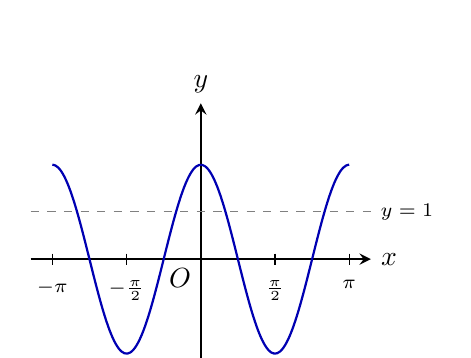
\begin{tikzpicture}[scale=0.6, >=stealth, baseline]
            \draw[->, thick] (-3.6, 0) -- (3.6, 0) node[right] {$x$};
            \draw[->, thick] (0, -2.3) -- (0, 3.3) node[above] {$y$};
            \foreach \x/\label in {-3.14159/{-\pi},-1.5708/{-\frac{\pi}{2}},1.5708/{\frac{\pi}{2}},3.14159/{\pi}} {
                \draw (\x,0.12) -- (\x,-0.12) node[below=2pt] {\scriptsize $\label$};
            }
            \draw[dashed, gray] (-3.6, 1) -- (3.6, 1);
            \draw[domain=-3.14159:3.14159, smooth, samples=100, thick, blue!70!black]
                plot (\x, {2*cos(2*\x r)});
            \node[below left] at (0,0) {$O$};
            \node[right] at (3.6, 1) {\scriptsize $y=1$};
        \end{tikzpicture}

        \item
        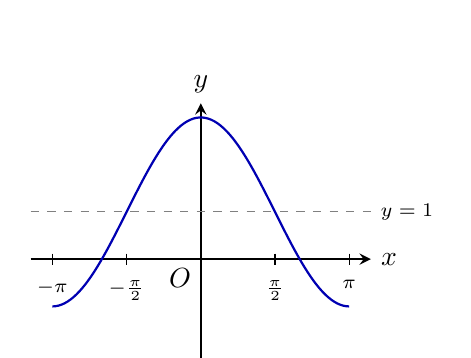
\begin{tikzpicture}[scale=0.6, >=stealth, baseline]
            \draw[->, thick] (-3.6, 0) -- (3.6, 0) node[right] {$x$};
            \draw[->, thick] (0, -2.3) -- (0, 3.3) node[above] {$y$};
            \foreach \x/\label in {-3.14159/{-\pi},-1.5708/{-\frac{\pi}{2}},1.5708/{\frac{\pi}{2}},3.14159/{\pi}} {
                \draw (\x,0.12) -- (\x,-0.12) node[below=2pt] {\scriptsize $\label$};
            }
            \draw[dashed, gray] (-3.6, 1) -- (3.6, 1);
            \draw[domain=-3.14159:3.14159, smooth, samples=100, thick, blue!70!black]
                plot (\x, {2*cos(\x r) + 1});
            \node[below left] at (0,0) {$O$};
            \node[right] at (3.6, 1) {\scriptsize $y=1$};
        \end{tikzpicture}

        \item
        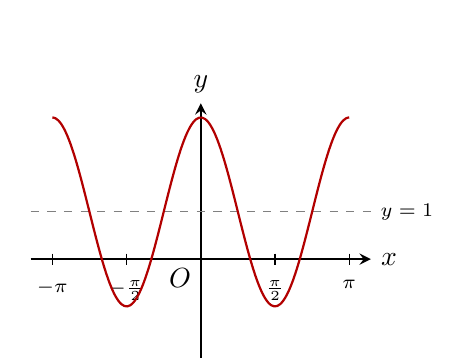
\begin{tikzpicture}[scale=0.6, >=stealth, baseline]
            \draw[->, thick] (-3.6, 0) -- (3.6, 0) node[right] {$x$};
            \draw[->, thick] (0, -2.3) -- (0, 3.3) node[above] {$y$};
            \foreach \x/\label in {-3.14159/{-\pi},-1.5708/{-\frac{\pi}{2}},1.5708/{\frac{\pi}{2}},3.14159/{\pi}} {
                \draw (\x,0.12) -- (\x,-0.12) node[below=2pt] {\scriptsize $\label$};
            }
            \draw[dashed, gray] (-3.6, 1) -- (3.6, 1);
            \draw[domain=-3.14159:3.14159, smooth, samples=100, thick, red!70!black]
                plot (\x, {2*cos(2*\x r) + 1});
            \node[below left] at (0,0) {$O$};
            \node[right] at (3.6, 1) {\scriptsize $y=1$};
        \end{tikzpicture}

        \item
        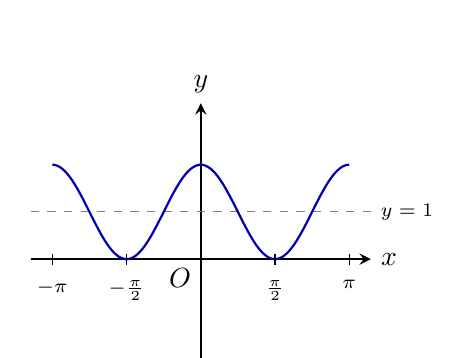
\begin{tikzpicture}[scale=0.6, >=stealth, baseline]
            \draw[->, thick] (-3.6, 0) -- (3.6, 0) node[right] {$x$};
            \draw[->, thick] (0, -2.3) -- (0, 3.3) node[above] {$y$};
            \foreach \x/\label in {-3.14159/{-\pi},-1.5708/{-\frac{\pi}{2}},1.5708/{\frac{\pi}{2}},3.14159/{\pi}} {
                \draw (\x,0.12) -- (\x,-0.12) node[below=2pt] {\scriptsize $\label$};
            }
            \draw[dashed, gray] (-3.6, 1) -- (3.6, 1);
            \draw[domain=-3.14159:3.14159, smooth, samples=100, thick, blue!70!black]
                plot (\x, {cos(2*\x r) + 1});
            \node[below left] at (0,0) {$O$};
            \node[right] at (3.6, 1) {\scriptsize $y=1$};
        \end{tikzpicture}
    \end{choices}
\end{question}

\begin{solution}
    需从四个选项中选出正确表示 $y = 2\cos 2x + 1$ 在 $[-\pi, \pi]$ 上图像的一项。 \\
    分别核对振幅、周期与垂直平移三项特征。
    \begin{align*}
        \text{振幅} &= 2, & T &= \frac{2\pi}{2}=\pi, \\
        \text{中心线} &: y=1
    \end{align*}
    只有选项 (C) 同时满足振幅为 $2$、周期为 $\pi$、图像沿 $y=1$ 振动这三项特征。
    故选 C。
\end{solution}
%endregion

%region 范围：高中数学·三角函数 | 考点：诱导公式与象限角三角函数值符号判断 | 难度：中等
\begin{question}
    已知 $\theta$ 为第三象限角，且 $\cos\theta = a$，求 $\cos\left(\theta + \dfrac{5\pi}{2}\right)$ 的值（用 $a$ 表示）。\paren[B]
    \begin{choices}
        \item $-\sqrt{1-a^2}$
        \item $\sqrt{1-a^2}$
        \item $-a$
        \item $a$
    \end{choices}
\end{question}

\begin{solution}
    已知 $\theta$ 为第三象限角，$\cos\theta=a$，求 $\cos\left(\theta+\dfrac{5\pi}{2}\right)$。 \\
    先化简角度，再用诱导公式转化为 $\sin\theta$，结合象限确定符号。
    \begin{align*}
        \cos\left(\theta+\frac{5\pi}{2}\right) &= \cos\left(\theta+\frac{\pi}{2}\right) \\
        &= -\sin\theta
    \end{align*}
    由 $\theta$ 为第三象限角知 $\sin\theta<0$，结合 $\sin^2\theta+\cos^2\theta=1$：
    \[
        \sin\theta=-\sqrt{1-a^2}
    \]
    \[
        \cos\left(\theta+\frac{5\pi}{2}\right) = -\sin\theta = \sqrt{1-a^2}
    \]
    故选 B。
\end{solution}
%endregion

%region 范围：高中数学·解三角形 | 考点：余弦定理逆用——由三边比例判断最大角 | 难度：中等
\begin{question}
    在 $\triangle ABC$ 中，三边长之比为 $a : b : c = 1 : \sqrt{3} : \sqrt{7}$。求该三角形中最大的角。\paren[D]
    \begin{choices}
        \item $90°$
        \item $120°$
        \item $135°$
        \item $150°$
    \end{choices}
\end{question}

\begin{solution}
    已知 $\triangle ABC$ 中 $a:b:c=1:\sqrt3:\sqrt7$，求最长边所对的角。 \\
    大边对大角，设 $a=1,b=\sqrt3,c=\sqrt7$，代入余弦定理求角 $C$。
    \begin{align*}
        \cos C &= \frac{a^2+b^2-c^2}{2ab} \\
        &= \frac{1+3-7}{2\sqrt3}
        = -\frac{\sqrt3}{2}
    \end{align*}
    由 $C\in(0°,180°)$，得
    \[
        C = 150°
    \]
    故选 D。
\end{solution}
%endregion

%region 范围：高中数学·解三角形 | 考点：三角形面积公式反推夹角与余弦定理求第三边（两解取舍） | 难度：中等偏难
\begin{question}
    在 $\triangle ABC$ 中，已知 $a = 4$，$b = 5$，且 $\triangle ABC$ 的面积为 $5\sqrt{3}$。若已知该三角形为钝角三角形，求第三边 $c$ 的长度。\paren[C]
    \begin{choices}
        \item $\sqrt{21}$
        \item $\sqrt{41}$
        \item $\sqrt{61}$
        \item $9$
    \end{choices}
\end{question}

\begin{solution}
    已知 $\triangle ABC$ 中 $a=4$，$b=5$，面积为 $5\sqrt3$，且为钝角三角形，求第三边 $c$。 \\
    先由面积公式求夹角 $C$，依钝角条件取舍，再用余弦定理求 $c$。
    \begin{align*}
        5\sqrt3 &= \frac12(4)(5)\sin C \\
        \sin C &= \frac{\sqrt3}{2} \\
        C &= 60°\ \text{或}\ 120°
    \end{align*}
    由三角形为钝角三角形，取 $C=120°$：
    \begin{align*}
        c^2 &= a^2+b^2-2ab\cos C \\
        &= 16+25-40\left(-\frac12\right) \\
        &= 61
    \end{align*}
    \[
        c=\sqrt{61}
    \]
    故选 C。
\end{solution}
%endregion


%region 范围：高中数学-二倍角公式与三角函数最值 | 考点：提取公因式后连续运用二倍角公式化简求最值 | 难度：基础
\begin{question}
    求函数 $f(\theta) = 2\left(\sin\theta\cos^3\theta - \sin^3\theta\cos\theta\right)$ 的最大值。 \paren[B]
    \begin{choices}
        \item $\dfrac{1}{4}$
        \item $\dfrac{1}{2}$
        \item $1$
        \item $2$
    \end{choices}
\end{question}

\begin{solution}
    求 $f(\theta) = 2\left(\sin\theta\cos^3\theta - \sin^3\theta\cos\theta\right)$ 的最大值。 \\
    先提取公因式化简，再连续运用二倍角公式。
    \begin{align*}
        f(\theta) &= 2\sin\theta\cos\theta\left(\cos^2\theta-\sin^2\theta\right) \\
        &= \sin2\theta\cos2\theta \\
        &= \frac{1}{2}\sin4\theta
    \end{align*}
    当 $\sin4\theta = 1$ 时，$f(\theta)$ 取得最大值 $\dfrac{1}{2}$。
    故选 B。
\end{solution}
%endregion
% %region 范围：高中数学·三角恒等变换 | 考点：三倍角公式展开与二倍角公式化简求最值 | 难度：中等偏难
% \begin{question}
%     求函数 $f(\theta) = 2\sin\theta\cos^3\theta - \sin3\theta\cos\theta$ 的最大值。\paren[A]
%     \begin{choices}
%         \item $\dfrac{1}{4}$
%         \item $\dfrac{1}{2}$
%         \item $1$
%         \item $-\dfrac{1}{4}$
%     \end{choices}
% \end{question}

% \begin{solution}
%     \textbf{解析：} \\
%     先利用三倍角公式 $\sin3\theta = 3\sin\theta - 4\sin^3\theta$ 将 $\sin3\theta\cos\theta$ 展开，代入原式：
%     \[ \displaystyle f(\theta) = 2\sin\theta\cos^3\theta - (3\sin\theta - 4\sin^3\theta)\cos\theta \]
%     \[ \displaystyle = 2\sin\theta\cos^3\theta - 3\sin\theta\cos\theta + 4\sin^3\theta\cos\theta \]

%     提取公因式 $\sin\theta\cos\theta$：
%     \[ \displaystyle f(\theta) = \sin\theta\cos\theta\left(2\cos^2\theta - 3 + 4\sin^2\theta\right) \]

%     利用同角关系 $\cos^2\theta = 1 - \sin^2\theta$ 将括号内式子统一为 $\sin^2\theta$ 的表达式：
%     \[ \displaystyle 2\cos^2\theta - 3 + 4\sin^2\theta = 2(1-\sin^2\theta) - 3 + 4\sin^2\theta = -1 + 2\sin^2\theta \]

%     再利用二倍角公式 $\cos2\theta = 1 - 2\sin^2\theta$，可知 $-1+2\sin^2\theta = -\cos2\theta$，故
%     \[ \displaystyle f(\theta) = \sin\theta\cos\theta \cdot (-\cos2\theta) = -\sin\theta\cos\theta\cos2\theta \]

%     再次利用二倍角公式 $\sin\theta\cos\theta = \dfrac{1}{2}\sin2\theta$，代入：
%     \[ \displaystyle f(\theta) = -\frac{1}{2}\sin2\theta\cos2\theta = -\frac{1}{4}\sin4\theta \]

%     （此处再次运用二倍角公式 $\sin2\theta\cos2\theta = \dfrac{1}{2}\sin4\theta$。）

%     由于 $\sin4\theta \in [-1, 1]$，当 $\sin4\theta = -1$ 时，$f(\theta)$ 取得最大值：
%     \[ \displaystyle f(\theta)_{\max} = -\frac{1}{4} \times (-1) = \frac{1}{4} \]

%     选项 (B) 是漏做了最后一步 $\sin2\theta\cos2\theta = \dfrac12\sin4\theta$ 的二倍角合并，误将 $-\dfrac12\sin4\theta$ 本身的振幅当作答案；选项 (C) 是同时漏掉了两次二倍角合并中的系数 $\dfrac12$，把振幅误算为 $1$；选项 (D) 则是符号判断错误，误取 $\sin4\theta=1$ 时的函数值作为最大值，实际上那对应的是函数的最小值。

%     故选 A。
% \end{solution}
% %endregion

%region 范围：高中数学·三角方程 | 考点：三角方程求解——因式分解法与两边同除丢根陷阱 | 难度：中等
\begin{question}
    求方程 $\tan x = 2\sin x$ 在区间 $[0, 2\pi)$ 内解的个数。\paren[C]
    \begin{choices}
        \item $2$
        \item $3$
        \item $4$
        \item $6$
    \end{choices}
\end{question}

\begin{solution}
    求方程 $\tan x=2\sin x$ 在 $[0,2\pi)$ 内解的个数。 \\
    化为正弦、余弦形式，两边同乘 $\cos x$（不可直接除以 $\sin x$，以免丢根），再因式分解求解。
    \begin{align*}
        \frac{\sin x}{\cos x} &= 2\sin x \\
        \sin x &= 2\sin x\cos x \\
        \sin x(1-2\cos x) &= 0
    \end{align*}
    \textbf{情况一：$\sin x=0$}
    \[
        x=0\ \text{或}\ x=\pi
    \]
    \textbf{情况二：$\cos x=\dfrac12$}
    \[
        x=\frac{\pi}{3}\ \text{或}\ x=\frac{5\pi}{3}
    \]
    四解均满足 $\cos x\neq0$，共 $4$ 个解。
    故选 C。
\end{solution}
%endregion

\newpage


%region 范围：高中数学-直线方程与斜率 | 考点：由直线一般式求斜率、点在直线上代入求参数 | 难度：中等
\begin{question}
    已知直线 $ax+by=2$ 的斜率为 $-\dfrac{1}{2}$，且经过点 $(4,1)$，求 $a+b$ 的值。 \paren[C]
    \begin{choices}
        \item $-1$
        \item $\dfrac{2}{3}$
        \item $1$
        \item $2$
    \end{choices}
\end{question}

\begin{solution}
    已知直线 $ax+by=2$ 的斜率为 $-\dfrac12$，且过点 $(4,1)$，求 $a+b$。 \\
    化为斜截式求出 $a,b$ 关系，再代入点坐标联立求解。
    \[
        y=-\frac{a}{b}x+\frac{2}{b} \implies -\frac{a}{b}=-\frac12 \implies a=\frac{b}{2}
    \]
    代入点 $(4,1)$：
    \begin{align*}
        4a+b &= 2 \\
        4\cdot\frac{b}{2}+b &= 2 \\
        3b &= 2
    \end{align*}
    解得 $b=\dfrac23$，$a=\dfrac13$。
    \[
        a+b=\frac13+\frac23=1
    \]
    故选 C。
\end{solution}
%endregion
% %region 范围：高中数学·直线与圆·距离公式 | 考点：由两定点距离之比求动点轨迹方程（阿波罗尼奥斯圆） | 难度：中等偏难
% \begin{question}
%     已知平面上两定点 $A(-1, 0)$ 与 $B(2, 0)$，动点 $P(x, y)$ 满足 $|PA| : |PB| = 1 : 2$，求点 $P$ 的轨迹方程。\paren[B]
%     \begin{choices}
%         \item $(x-2)^2 + y^2 = 4$
%         \item $(x+2)^2 + y^2 = 4$
%         \item $(x+2)^2 + y^2 = 16$
%         \item $(x-\frac{1}{3})^2 + y^2 = \frac{4}{3}$
%     \end{choices}
% \end{question}

% \begin{solution}
%     \textbf{解析：} \\
%     设动点 $P(x, y)$，由距离公式分别写出 $|PA|^2$ 与 $|PB|^2$：
%     \[ \displaystyle |PA|^2 = (x+1)^2 + y^2, \qquad |PB|^2 = (x-2)^2 + y^2 \]

%     由条件 $|PA| : |PB| = 1 : 2$，即 $|PB| = 2|PA|$，两边平方（避免根号，直接用距离平方之比处理）：
%     \[ \displaystyle |PB|^2 = 4|PA|^2 \]

%     代入并展开：
%     \[ \displaystyle (x-2)^2 + y^2 = 4\left[(x+1)^2 + y^2\right] \]
%     \[ \displaystyle x^2 - 4x + 4 + y^2 = 4x^2 + 8x + 4 + 4y^2 \]

%     移项整理，将所有项集中到等式一侧：
%     \[ \displaystyle x^2 - 4x + 4 + y^2 - 4x^2 - 8x - 4 - 4y^2 = 0 \]
%     \[ \displaystyle -3x^2 - 12x - 3y^2 = 0 \]

%     两边同除以 $-3$：
%     \[ \displaystyle x^2 + 4x + y^2 = 0 \]

%     对 $x$ 项配方：
%     \[ \displaystyle (x^2 + 4x + 4) + y^2 = 4 \]
%     \[ \displaystyle (x+2)^2 + y^2 = 4 \]

%     因此点 $P$ 的轨迹是以 $(-2, 0)$ 为圆心、半径为 $2$ 的圆。

%     选项 (A) 是把比值方向搞反，误设为 $|PA| = 2|PB|$（即误解为 $|PA|:|PB|=2:1$），导致配方后圆心落在 $B$ 一侧的 $(2,0)$；选项 (C) 是配方时半径计算错误，把 $4$ 误写为常数项 $16$，忽略了配方补齐的系数关系；选项 (D) 则是在两边平方或移项过程中系数处理错误，未能正确合并 $x^2$ 项系数，导致圆心与半径均计算失真。

%     故选 B。
% \end{solution}
% %endregion

%region 范围：高中数学·平面向量与坐标几何 | 考点：外分点公式的应用与内分/外分公式混淆辨析 | 难度：中等偏难
\begin{question}
    已知两点 $A(a, 2)$ 与 $B(4, b)$。若点 $C(10, -1)$ 是线段 $AB$ 延长线上的外分点，且满足 $AC : CB = 3 : 1$，求 $a + b$ 的值。\paren[A]
    \begin{choices}
        \item $-8$
        \item $-4$
        \item $4$
        \item $8$
    \end{choices}
\end{question}

\begin{solution}
    已知 $A(a,2)$，$B(4,b)$，外分点 $C(10,-1)$ 满足 $AC:CB=3:1$，求 $a+b$。 \\
    设 $m=3,n=1$，代入外分点公式
    \[
        C=\left(\frac{mB_x-nA_x}{m-n},
        \frac{mB_y-nA_y}{m-n}\right)
    \]
    求坐标。
    \begin{align*}
        10 &= \frac{3(4)-a}{2} \implies a=-8 \\
        -1 &= \frac{3b-2}{2} \implies b=0
    \end{align*}
    \[
        a+b=-8+0=-8
    \]
    故选 A。
\end{solution}
%endregion


%region 范围：高中数学·平面直角坐标系与多边形面积 | 考点：鞋带公式应用——顶点连接顺序的判断与重新排列 | 难度：困难
\begin{question}
    在直角坐标系中，四边形的四个顶点坐标分别为 $M(1, 5)$、$N(-2, -3)$、$P(-3, 2)$、$Q(3, -1)$。求该四边形的面积。\paren[C]
    \begin{choices}
        \item $3.5$
        \item $14.5$
        \item $28.5$
        \item $57$
    \end{choices}
\end{question}

\begin{solution}
    求四边形 $MNPQ$（$M(1,5)$，$N(-2,-3)$，$P(-3,2)$，$Q(3,-1)$）的面积。 \\
    先按顶点实际位置确定正确连接顺序，再代入鞋带公式。
    \[
        M\to P\to N\to Q\to M
    \]
    \begin{align*}
        S &= \frac12\left|
        \begin{aligned}
          &(x_My_P+x_Py_N)+(x_Ny_Q+x_Qy_M)\\
          &-(y_Mx_P+y_Px_N)-(y_Nx_Q+y_Qx_M)
        \end{aligned}
        \right| \\
        &= \frac12\big|(2+9+2+15)-(-15-4-9-1)\big| \\
        &= \frac12|28-(-29)| \\
        &= 28.5
    \end{align*}
    故选 C。
\end{solution}
%endregion

%region 范围：高中/大学预备微积分·微分的应用 | 考点：隐函数求导法求曲线切线斜率 | 难度：中等偏难
\begin{question}
    已知曲线方程为 $x^3 + xy + y^3 = 3$，求该曲线在 $x = 1$ 处的切线斜率。\paren[B]
    \begin{choices}
        \item $-7$
        \item $-1$
        \item $-\dfrac{3}{4}$
        \item $\dfrac{3}{4}$
    \end{choices}
\end{question}

\begin{solution}
    求曲线 $x^3+xy+y^3=3$ 在 $x=1$ 处的切线斜率。 \\
    先求切点纵坐标，再用隐函数求导法求 $\dfrac{dy}{dx}$。
    \begin{align*}
        1+y+y^3 &= 3 \\
        (y-1)(y^2+y+2) &= 0 \\
        y &= 1
    \end{align*}
    两边对 $x$ 求导（$xy$ 项用乘积法则，$y^3$ 项用链式法则）：
    \[
        3x^2+\left(y+x\frac{dy}{dx}\right)+3y^2\frac{dy}{dx}=0
    \]
    \[
        \frac{dy}{dx}=\frac{-(3x^2+y)}{x+3y^2}
    \]
    代入 $(1,1)$：
    \[
        \frac{dy}{dx}=\frac{-(3+1)}{1+3}=-1
    \]
    故选 B。
\end{solution}
%endregion

%region 范围：高中/大学预备微积分·导数的应用 | 考点：利用二阶导数判别法求函数极大值 | 难度：中等
\begin{question}
    已知函数 $f(x) = x + \dfrac{4}{x}$（$x \neq 0$），求 $f(x)$ 的极大值。\paren[A]
    \begin{choices}
        \item $-4$
        \item $-2$
        \item $2$
        \item $4$
    \end{choices}
\end{question}

\begin{solution}
    求 $f(x)=x+\dfrac4x$（$x\neq0$）的极大值。 \\
    先求驻点，再用二阶导数判别法确定极大值点。
    \[
        f'(x)=1-\frac{4}{x^2}=0 \implies x=2\ \text{或}\ x=-2
    \]
    \[
        f''(x)=\frac{8}{x^3}
    \]
    \begin{align*}
        f''(2) &= 1>0 \implies x=2\ \text{为极小值点} \\
        f''(-2) &= -1<0 \implies x=-2\ \text{为极大值点}
    \end{align*}
    \[
        f(-2)=-2+\frac{4}{-2}=-4
    \]
    故选 A。
\end{solution}
%endregion

%region 范围：高中/大学预备微积分·相关变化率 | 考点：链式法则求面积随时间的变化率 | 难度：中等
\begin{question}
    一圆形薄片的半径以 $2\text{ cm/s}$ 的速率减少。当该圆的直径为 $20\text{ cm}$ 时，求其面积改变的速率。\paren[B]
    \begin{choices}
        \item $-80\pi \text{ cm}^2/\text{s}$
        \item $-40\pi \text{ cm}^2/\text{s}$
        \item $-20\pi \text{ cm}^2/\text{s}$
        \item $40\pi \text{ cm}^2/\text{s}$
    \end{choices}
\end{question}

\begin{solution}
    圆形薄片半径以 $2\text{ cm/s}$ 减少，直径为 $20\text{ cm}$ 时，求面积改变的速率。 \\
    设 $A=\pi r^2$，用链式法则对 $t$ 求导。
    \[
        \frac{dr}{dt}=-2,\qquad r=\frac{20}{2}=10
    \]
    \begin{align*}
        \frac{dA}{dt}
        &= \frac{dA}{dr}\cdot\frac{dr}{dt} \\
        &= 2\pi r\cdot\frac{dr}{dt} \\
        &= 2\pi(10)(-2) \\
        &= -40\pi\ \text{cm}^2/\text{s}
    \end{align*}
    故选 B。
\end{solution}
%endregion

%region 范围：高中/大学预备微积分·闭区间上函数的最大值 | 考点：利用导数求闭区间上多项式函数的最大值（临界点与端点比较法） | 难度：中等
\begin{question}
    已知函数 $f(x) = x^3 - 3x^2 - 9x + 5$，求 $f(x)$ 在闭区间 $[-2, 4]$ 上的最大值。\paren[D]
    \begin{choices}
        \item $-22$
        \item $-15$
        \item $3$
        \item $10$
    \end{choices}
\end{question}

\begin{solution}
    求 $f(x)=x^3-3x^2-9x+5$ 在 $[-2,4]$ 上的最大值。 \\
    先求临界点，再比较临界点与端点处的函数值。
    \begin{align*}
        f'(x) &= 3x^2-6x-9=0 \\
        (x-3)(x+1) &= 0 \\
        x &= 3\ \text{或}\ x=-1
    \end{align*}
    \begin{align*}
        f(-2) &= -8-12+18+5=3 \\
        f(-1) &= -1-3+9+5=10 \\
        f(3) &= 27-27-27+5=-22 \\
        f(4) &= 64-48-36+5=-15
    \end{align*}
    比较四值，最大值为
    \[
        f(x)_{\max}=f(-1)=10
    \]
    故选 D。
\end{solution}
%endregion

%region 范围：高中/大学预备微积分·不定积分 | 考点：利用三角恒等式转换被积函数求不定积分 | 难度：中等
\begin{question}
    求不定积分 $\displaystyle\int \tan^2 x\,dx$。\paren[A]
    \begin{choices}
        \item $\tan x - x + C$
        \item $\dfrac{1}{3}\tan^3 x + C$
        \item $\sec^2 x - x + C$
        \item $-\tan x - x + C$
    \end{choices}
\end{question}

\begin{solution}
    求 $\displaystyle\int\tan^2x\,dx$。 \\
    利用恒等式 $\tan^2x=\sec^2x-1$ 转化被积函数，再逐项积分。
    \[
        \int\tan^2x\,dx=\int(\sec^2x-1)\,dx=\tan x-x+C
    \]
    故选 A。
\end{solution}
%endregion

%region 范围：高中/大学预备微积分·换元积分法 | 考点：换元积分法（$u$-替换）中系数处理 | 难度：中等
\begin{question}
    求不定积分 $\displaystyle\int x^2(x^3+1)^4\,dx$。\paren[A]
    \begin{choices}
        \item $\dfrac{(x^3+1)^5}{15} + C$
        \item $\dfrac{(x^3+1)^5}{5} + C$
        \item $\dfrac{(x^3+1)^4}{12} + C$
        \item $x^2 \cdot \dfrac{(x^3+1)^5}{15} + C$
    \end{choices}
\end{question}

\begin{solution}
    求 $\displaystyle\int x^2(x^3+1)^4\,dx$。 \\
    设 $u=x^3+1$，用换元积分法求解。
    \[
        u=x^3+1 \implies du=3x^2\,dx \implies x^2\,dx=\frac13\,du
    \]
    \begin{align*}
        \int x^2(x^3+1)^4\,dx &= \frac13\int u^4\,du \\
        &= \frac13\cdot\frac{u^5}{5}+C \\
        &= \frac{(x^3+1)^5}{15}+C
    \end{align*}
    故选 A。
\end{solution}
%endregion

%region 范围：高中/大学预备微积分·部分分式积分法 | 考点：部分分式分解与对数函数积分公式的综合应用 | 难度：中等偏难
\begin{question}
    求不定积分 $\displaystyle\int \frac{x+7}{(x-1)(x+3)}\,dx$。\paren[B]
    \begin{choices}
        \item $\ln|x-1| - 2\ln|x+3| + C$
        \item $2\ln|x-1| - \ln|x+3| + C$
        \item $2\ln|x-1| + \ln|x+3| + C$
        \item $\dfrac{1}{2}\ln|x-1| - \dfrac{1}{3}\ln|x+3| + C$
    \end{choices}
\end{question}

\begin{solution}
    求 $\displaystyle\int\frac{x+7}{(x-1)(x+3)}\,dx$。 \\
    用部分分式法拆分被积函数，再逐项积分。
    \begin{align*}
        \frac{x+7}{(x-1)(x+3)}
        &= \frac{A}{x-1}+\frac{B}{x+3} \\
        x+7 &= A(x+3)+B(x-1)
    \end{align*}
    \begin{align*}
        x=1:&\quad 8=4A \implies A=2 \\
        x=-3:&\quad 4=-4B \implies B=-1
    \end{align*}
    \begin{align*}
        \int\left(\frac{2}{x-1}-\frac{1}{x+3}\right)dx
        &= 2\ln|x-1| \\
        &\quad -\ln|x+3|+C
    \end{align*}
    故选 B。
\end{solution}
%endregion
\vfill % 与上方内容保持距离

\noindent
\newlength{\sigwidth}
\settowidth{\sigwidth}{（\hspace{4em}师）}

\begin{tabular*}{\textwidth}{@{\extracolsep{\fill}} l l l}
    出题： & 审题： & 审核： \\[4em]
    \rule{\sigwidth}{0.5pt} &
    \rule{\sigwidth}{0.5pt} &
    \rule{\sigwidth}{0.5pt} \\
    （\hspace{0em} \setterteacher ） &
    （\hspace{0em} \reviewteacher ）  &
    （\hspace{0em} \auditteacher ） \\
\end{tabular*}

\clearpage
\thispagestyle{empty} % 取消这一页的页眉页脚（页码）
~
\clearpage
\end{document}